% !TEX root = ./Vorlesungsmitschrift DIFF 2.tex  
\lecture{Mo 13.07. 10:15}{}
Letztes Mal: Satz von Gauß
\begin{bemerkungen*}
  \begin{enumerate}[label=\rechtsklammer{\arabic*}, ref=Bemerkung \rechtsklammer{\arabic*}]
    \item \label{komponentenweiser_satz_von_gauss}Tatsächlich gilt die Gleichung sogar komponentenweise, also für \( f\in \stetigefunktionen[1](G,\reals) \) gilt
    \begin{equation*}
      \Integrate{\partial_i f(x)}{x,G}=\Integrate{f(x) \nu_i(x)}{S(x),\randpunkte{G}}.
    \end{equation*}
    \item Der Satz gilt immer noch, wenn \( \randpunkte{G} \) höchstens \( (n-2) \)-dimensionale \enquote{Kanten} und \enquote{Ecken} hat, in denen glatte Stücke von \( randpunkte{G} \) zusammentreffen, also insbesondere auch für Quader.
    \item Aus \ref{komponentenweiser_satz_von_gauss} folgt sofort: Ist \( \supp X\subset \inneres{G} \) so ist \( \Integrate{\div X}{x,C}=0 \).
  \end{enumerate}
\end{bemerkungen*}
Physikalische Interpretation \tto Vorlesung 23: Quellstärke im Inneren \teq Fluss durch die Oberfläche. Physikalische und mathematische Anwendung:
\begin{beispiele}
  \begin{enumerate}
    \item Elektrodynamik: \( \Integrate{\div E(x)}{x,G} =\Integrate{\scalarproduct{E}{\nu}}{S(x),\randpunkte{G}} \), \( \divergence{\explain[Big]{\text{elektrisches Feld}}{E(x)}}=\frac{1}{\explain{\text{konstant}}{\varepsilon_0}}\rho(x) \) (Maxwell-Gesetz), \( \rho \) Ladungsdichte (\( \rho(x) =\quotient{\text{Ladung}}{\text{Volumen}}\) an der Stelle \( x \)) \timplies \( \frac{Q}{\varepsilon_0}=\Integrate{\scalarproduct{E}{\nu}}{S(x),\randpunkte{G}} \), \( Q \) \teq Gesamtladung in \( G \). Aus dieser Gleichung kann man in vielen Fällen \( E \) berechnen.
    \item \begin{align*}
      \operatorname{vol}_{n-1}(\sphere{n-1})&=\Integrate{1}{S(x),\sphere{n-1}}\\
      &\explain[big]{\text{für \( X(x)=x \) (denn \( \nu(x)=x \) und \( \euclidiannorm{x}^2=1 \))}}{=}\Integrate{\scalarproduct{X(x)}{\nu(x)}}{S(x),\sphere{n-1}}\\
      &\explain[big]{\text{Gauß}}{=}\Integrate{\braceannotate{=n}{\divergence{X(x)}}}{x,\ball{1}{0}}.
    \end{align*}
    \( \sphere{n-1} \) \( (n-1) \)-dimensionale Einheitssphäre \tsubset \( \reals^n \), \( \ball{1}{0} \) Vollkugel von Radius \( 1 \) \tsubset \( \reals^n \).
  \end{enumerate}
\end{beispiele}
\begin{proof}[Beweis des Satzes (\vgl Forster. Analysis 3, Vieweg)]
  Wir beweisen die Behauptung aus \ref{komponentenweiser_satz_von_gauss}, aus der der Satz folgt.

  Sei \( U\subset \reals^n \) offen mit \( G \). Wähle zu \( x\in G \) eine offene Umgebung \( U_x\subset U \). Ist \( x\in \randpunkte{G} \) wähle \( U_x=\braceannotate{\mathclap{\text{\( (n-1) \)-dimensionaler Qauder}}}{U_x'}\times \overbrace{U_x''}^{\mathclap{\text{Intervall}}} \) \sd \texists \( \varphi\maps U_x'\to U_x'' \) \( \stetigefunktionen[1] \) (als Abbildung nach \( \reals \)) mit 
  \begin{align*}
    G\cap (U_x'\times U_x'')&=\Set{y\in U_x|y_n<\varphi(y')}\\
    \randpunkte{G}\cap (U_x'\times U_x'')&=\Set{y\in U_x|y_n=\varphi(y')}.
  \end{align*}
  \begin{figure}[H]
    \centering
    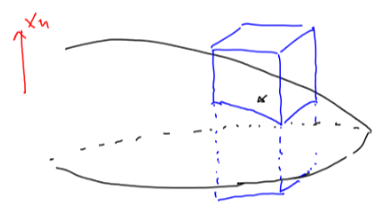
\includegraphics[width=0.5\linewidth]{satz_von_gauss_beweis_lokale_umgebung}
    \label{fig:satz_von_gauss_beweis_lokale_umgebung}
  \end{figure}
  \begin{beispiel*}[Sphäre]
    \begin{gather*}
      \varphi(x,y)=\sqrt{1-x^2-y^2}\\
      \Set{(x,y)|z=\phi(x,y)}=\square \subset D.
    \end{gather*}
  \end{beispiel*}
  Dann gilt: \( G\subset \bigcup_{x\in G}U_x \). \( G \) ist kompakt, denn nach Voraussetzung beschränkt und zudem abgeschlossen, da der topologische Rand (der \emph{hier} gleich dem geometrischen Rand ist) in \( G \) enthalten ist. \timplies \texists \( U_1,\dotsc,U_k \) (\( U_j=U_{x_j} \)) \sd \( G\subset \bigcup_{j=1}^k U_j \). Seien die \( U_j \) so nummeriert, dass
  \begin{gather*}
    U_j\cap \randpunkte{G}\neq \emptyset\quad 1\leq L\\
    U_j\subset G \quad L+1\leq j\leq K.
  \end{gather*}
  Wähle eine Partition der Eins \( \set{\rho_j}_{j\in \set{1,\dotsc,K}} \) mit \( \supp \rho_j\subset U_j \), \( \sum_{j=1}^{K}\rho_j(x)=1\quad \forall x\in G \).
  \begin{equation*}
    \implies \Integrate{\partial_i X_i(x)}{x,G}=\sum_{j=1}^{K}\Integrate{\partial_i\p*{\rho_j X_i}(x)}{x,G\cap U_j}
  \end{equation*}
  und
  \begin{equation*}
    \Integrate{X_i(x)v_i(x)}{S(x),\randpunkte{G}}=\sum_{j=1}^{K}\Integrate{\p*{\rho_j X_i v_i}(x)}{S(x),\randpunkte{G}\cap U_j}.
  \end{equation*}
  Wir zeigen also, dass \tforall \( j \), \( 1\leq j\leq L \), und \tforall \( F\in \explain{\text{\( \stetigefunktionen[1] \) und kompakter Träger}}{\stetigefunktionen[1]_{C}(U_j)} \) gilt
  \begin{equation*}
    \Integrate{\partial_i F}{x, G\cap U_j}=\Integrate{F \nu_i}{S(x),\randpunkte{G}\cap U_j}\tag{\( * \)}\label{eq:satz_von_gauss_beweis_randteil}
  \end{equation*}
  und \tforall \( j \), \( L+1\leq j\leq K \), und \tforall \( F\in \stetigefunktionen[1]_C(U_j) \) gilt
  \begin{equation}
      \tag{\( ** \)}\label{eq:satz_von_gauss_beweis_gesamtteil}
      \Integrate{\partial_i F}{x,G\cap U_j}=0
  \end{equation}

  Zu \eqref{eq:satz_von_gauss_beweis_gesamtteil}: Wähle \( A>0 \) so, dass \( \interval{-A}{A}^n\supset U_j \).
  \( \supp F\subsetneq U_j\Rightarrow \) kann durch 0 stetig differenzierbar zu \( \bar{F} \) auf \( \interval{-A}{A}^n \) fortgesetzt werden.
  \begin{equation*}
      \implies \Integrate{\partial_i F}{x,G\cap U_j}
      \explain[big]{\text{{\hyperref[fubini]{Fubini}}}}{=}
      \int_{-A}^{A}\dotsi \p*{ \underbrace{\int_{-A}^{A}\partial_i\bar{F}(x)  }_{=\evaluatebetween{\bar{F}(x)}{x_i=-A}{x_i=A}}
      \differential{x_1}}\differential{x_1}\cdots\explain{\text{fehlt}}{\widehat{\differential{x_i}}}\cdots\differential{x_n}=0
  \end{equation*}
  Zu \eqref{eq:satz_von_gauss_beweis_randteil}: Zunächst für \( 1\leq i\leq n-1 \):
  \begin{equation*}
      \Integrate{\partial_i F }{x,{G\cap U_j}} \overset{\text{\hyperref[fubini]{Fubini}}}{=}
      \int_{U_j'}\int_{a}^{\varphi(x')}\partial_i F(x',x_n)\differential{x_n}\differential{x'}
  \end{equation*}
  mit \( a=\inf U_{j}'' \).
  Es gilt:
  \begin{equation*}
      \int_{a}^{\varphi(x')} \partial_i F(x',x_n)\differential{x_n}=\partial_i\int_{a}^{\varphi(x')}F\differential{x_n}-F(x',\varphi(x'))\cdot \partial_i\varphi(x')
  \end{equation*}
  (siehe unten). Weiterhin gilt 
  \begin{align*}
      \int_{U_j'}\partial_i\p*{ \int_{a}^{\varphi(x')}F\differential{x_n} }\differential{x'} &= \int_{U^1_j\times \dotsb \times \widehat{U_j^i}\times \dotsb \times U_j^{n-1}}
      \underbrace{\int_{\inf U_j^i}^{\sup U_j^i}\partial_i\int_{a}^{\varphi(x')}F\differential{x_n}\differential{x_i}\differential{x_{1\ldots \widehat{i}\ldots }}
      }_{\begin{aligned}
          &= \int_{a}^{\varphi(\sup U_j^i)}
          \underbrace{F(x)\big|_{x_i=\sup U_j^i}}_{=0}\differential{x_n}\\
          &-\int_{a}^{\varphi(\inf U_j^i)}
          \underbrace{F(x)\big|_{x_i=\inf U_j^i}}_{=0}\differential{x_n}
      \end{aligned}
      }\\
      &= 0
  \end{align*}
  \begin{gather*}
      \implies \Integrate{\partial_i F}{x,{G\cap U_j}}\overset{\text{\hyperref[fubini]{Fubini}}}{=}
      \int_{U_j'}\int_{a}^{\varphi(x')}\partial_i F(x',x_n)\differential{x_n}\differential{x'}\\
      =\Integrate{F(x',\varphi(x'))\underbrace{\p*{ -\partial_i\varphi(x') }}_{\mathclap{=\nu_i(x',\varphi(x'))\sqrt{1+\norm{\grad-\varphi(x')}^2}}}}{x',{U_j'}}
      \intertext{denn (\s letzte Vorlesung)}
      \nu(a)=\frac{1}{\sqrt{1+\norm{\grad-\varphi(a')}^2}} \begin{pmatrix} -\grad-\varphi(a')\\1 \end{pmatrix} \qquad a=(a',a_n)  \end{gather*}
  Nun für \( i=n \):
  Hauptsatz der Differential- und Integralrechnung
  \begin{gather*}
      \implies \Integrate{\partial_n F}{x,{G\cap U_j}}=\int_{U_j'}\int_{a}^{\varphi(x')}\partial_n F(x',x_n)\differential{x_n}\differential{x'}\\
      =\int_{U_j}\big(\underbrace{F(x',\varphi(x'))}_
      {\begin{aligned}[t]
          =F\cdot \nu_n(x',\varphi(x'))\\\cdot \sqrt{1+\euclidiannorm{\grad-\varphi(x')}^2}            
      \end{aligned}
      }
      -\underbrace{F(x',a)}_{=0}\big)\differential{x'}
  \end{gather*}
  \timplies Beh.
\end{proof}

\begin{bemerkung*}
\begin{equation*}
    \int_{a}^{\varphi(x')}\partial_i F(x',x_n)\differential{x_n}=\partial_i\int_{a}^{\varphi(x')}F\differential{x_n}-F(x',\varphi(x'))\cdot \partial_i\varphi(x')
\end{equation*}
\diffcourse{1}: \emph{Parameterabhängige Integrale}.
Seien \( I,J \) kompakte Intervalle, \( f\maps I\times J\to \reals \) stetig.
\( \partial_1f \) existiere und sei stetig.
Dann ist 
\begin{equation*}
    I\ni x \mapsto g(x)\definedas \Integrate{ f(x,y)}{y,J}
\end{equation*}
stetig differenzierbar und es gilt:
\begin{equation*}
    g'(x)=\int_J\partial_1f(x,y)\differential{y}
\end{equation*}
siehe z.B. Forster, Analysis 2, Kap. I, §9. Satz 2 (1982).
Hängt die obere Integrationsgrenze von \( x \) ab, so gilt für \( \underline{g}(x,a)=F_2(x,a) \) (Stammfunktion von \( f \) bezüglich der 2. Variable ausgewertet in der Grenze \( a \))
\begin{gather*}
    \odv*{\p*{ \underline{g}(x,\varphi(x)) - \underline{g}(x,a) }}{x}= D\underline{g}(x,\varphi(x))\begin{pmatrix} 1\\\varphi'(x) \end{pmatrix} -Dg(x,a)\begin{pmatrix} 1\\0 \end{pmatrix} \\
    =g'(x)+\partial_2\underline{g}(x,\varphi(x))\cdot \varphi'(x)=\underbrace{g'(x)}_{\mathclap{\int_{a}^{\varphi(x)}\partial_1f(x,y)\differential{y}}}+f(x,\varphi(x))\varphi'(x)
\end{gather*}
\end{bemerkung*}

\begin{folgnotation}
Sei \( G\subset\reals^2 \) \( 2 \)-dimensionale beschränkte Untermannigfaltigkeit mit Rand.
Dann gilt für \( f,-g\in \stetigefunktionen[1](U) \), \(  U\supset G \):
\begin{equation*}
   \int_{G}\p*{ \partial_1g-\partial_2f }\differential{x}=\int_{\partial G}f\differential{x_1}+g\differential{x_2}
\end{equation*}
\enquote{Satz von Gauss} (einer der vielen)

rechte Seite: \begin{align*}
    \gamma(t)&= \begin{pmatrix} x(t)\\y(t) \end{pmatrix} \\
    \underline{\nu}(t)&= \begin{pmatrix} y'(t)\\-x'(t) \end{pmatrix} 
\end{align*}
\begin{figure}[H]
  \centering
  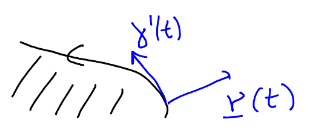
\includegraphics[width=0.5\linewidth]{normale_auf_rand}
  \label{fig:normale_auf_rand}
\end{figure}
mehr später.
\end{folgnotation}

\begin{beispiel}
\begin{equation*}
    I=\int_G 2(x+y)\differential{x}+(x^2+y^2)\differential{y}
\end{equation*}
\( C= \) bestehend aus 2 Teilkurven
\begin{gather*}
    \begin{aligned}[t]
        C_1:y&=-\sqrt{2x-x^2}\\
        C_2:y&=\frac{1}{2} \sin(\pi x)\quad x\in \interval{0}{2}            
    \end{aligned}\\
    I=\int_{0}^{2}\int_{-\sqrt{2x-x^2}}^{\frac{1}{2}\sin\pi x}(2x-2)\differential{y}\differential{x}=\dotsb =-\frac{2}{\pi} 
\end{gather*}
\begin{achtung*}
    Die Voraussetzungen sind wichtig:
    \( G=\overline{D} \) (Einheitskreisscheibe)
    \begin{gather*}
        f=-\frac{y}{x^2+y^2} \qquad g=\frac{x}{x^2+y^2} \\
        \int_G\underbrace{(\partial_1g-\partial_2f)}_{=0}\differential{(x,y)}=0 \neq \int_{\partial G}f\differential{x}+g\differential{y}.
    \end{gather*}
\end{achtung*}
\end{beispiel}

\section{Tensorkalkül und Differentialformen}
Lineare Algebra: Sei \( V \) ein \( n \)-dimensionaler Vektorraum.
Sei \( (e_1,\ldots ,e_n) \) eine Basis von \( V \). 
Dann gibt es eine eindeutig bestimmte Basis \( (e^1,\ldots ,e^n) \) von \( \dualspace{V} \), dem Dualraum, \( \dualspace{V}=L(V,\reals)=\Set{W\maps V\to\reals \text{ linear} } \)
\sd 
\begin{equation*}
e^j(e_i)=\delta_i^j=\begin{cases}
    1 & i=j\\
    0 & i\neq j
\end{cases}
\end{equation*}

Sie wird \enquote{\define{duale Basis}} genannt.

\begin{definition}
Seien \( V_1,\dotsc ,V_k,W \) Vektorräume. \index{multilineare Abbildung}
Eine Abbildung \( \alpha\maps V_1\times \dotsb \times V_k\to W \) heißt \emph{multilinear}, wenn sie in jeder Komponente linear ist.
Im Fall \( W=\reals \) heißt sie \define{Multilinearform}.

Seien \( r,s\in \naturals_0 \) (nicht beide gleich 0).
Ein \( r \)-fach kovarianter, \( s \)-fach kontravarianter \define{Tensor} ist eine multilineare Abbildung
\begin{equation*}
    \alpha\maps \underbrace{V\times \dotsb \times V}_{\text{\( r \)-fach}}\times 
    \underbrace{\dualspace{V}\times \dotsb \times \dualspace{V}}_{\text{\( s \)-fach}}
    \to\reals.
\end{equation*}
\( T_r^s(V) \) bezeichnet den Vektorraum der \( r \)-fach ko- und \( s \)-fach kontravarianten Tensoren.
\end{definition}

\begin{definition}
Sei \( \alpha\in T_r^s(V),\quad \beta\in T_{\tilde{r}}^{\tilde{s}}(V) \).
Dann ist \( \alpha\otimes\beta \) erklärt durch \( (v_i\in V,w^j\in \dualspace{V}) \)
\begin{gather*}
    \alpha\otimes\beta(v_1,\ldots ,v_r,v_{r+1},\ldots ,v_{r+\tilde{r}},
    w^1,\ldots ,w^s,w^{s+1},\ldots ,w^{s+\tilde{s}})\\
    \definedas \alpha(v_1,\ldots ,v_r,w^1,\ldots ,w^s)\cdot 
    \beta(v_{r+1},\ldots ,w_{r+\tilde{r}},w^{s+1},\ldots ,w^{s+\tilde{s}})
\end{gather*}
\end{definition}

\begin{beispiel*}
\( \alpha\in \dualspace{V} \) ist ein 1-fach kovarianter Tensor.

\( \scalarproduct{\cdot}{\cdot}\maps V\times V\to\reals \) ist ein 2-fach kovarianter Tensor.

\( \determinant\maps V^n\to\reals \) (als Abbildung auf dem Spaltenvektoren, \( V \) \( n \)-dimensional) ist ein \( n \)-fach kovarianter Tensor.

\( v\in V \) ist ein 1-fach kontravarianter Tensor:
\( v\in V\cong V^{**} \) mit \( v(\alpha)\definedas \alpha(v),\quad \alpha\in \dualspace{V} \).
\end{beispiel*}

\begin{satz}\label{basis_tensorraum}
Sei \( (e_i)_{i\in\set{1,\ldots ,n}} \) Basis von \( V \), sei \( (e^j)_j \) die duale Basis (von \( \dualspace{V} \)).
Dann ist 
\begin{equation*}
    \Set{e^{j_1}\otimes\ldots \otimes e^{j_r}\otimes e_{i_1}\otimes\ldots \otimes e_{i_s}| j_l,i_k\in\set{1,\ldots ,n} }
\end{equation*}
eine Basis von \( T^s_r(V) \).
Somit ist \( \dim T^s_r(V)=n^{r+s} \).    
\end{satz}

\begin{proof}[Beweis (wird in der Vorlesung eventuell weggelassen)]
Wir setzen \( s=0 \) (der Beweis für \( s>0 \) verläuft analog).
Es gilt:
\begin{gather*}
    (e^{j_1}\otimes e^{j_r})(e_{k_1},\ldots ,e_{k_r})=\delta_{k_1}^{j_1}\cdots \delta_{k_r}^{j_r}
    =\begin{cases}
        1 & (j_1,\ldots ,j_r)=(k_1,\ldots ,k_r)\\
        0 & \text{sonst}
    \end{cases}\\
    \implies \text{Falls }\sum \underbrace{c_{j_n\cdots j_r}}_{\in\reals}e^{j_1}\otimes \ldots \otimes e^{j_r}=0
\end{gather*}
so sind alle \( c_{j_1\cdots j_r}=0 \).

ist \( \alpha\in T_r(V) \), setze für alle Kombinationen \( (k_1,\ldots ,k_r)\in\set{1,\ldots ,n}^r \)
\begin{equation*}
    \alpha_{k_1\cdots k_r}\definedas \alpha(e_{k_1},\ldots ,e_{k_r}).
\end{equation*}
Dann gilt für \( u_1,\ldots ,u_r\in V \):
\begin{align*}
    \alpha(u_1,\ldots ,u_r)&= \alpha\p*{ \sum u_1^j e_j,\ldots ,\sum u_r^j e_j }\\
    &= \sum_{k_1,\ldots ,k_r}u_1^{k_1}\cdots u_1^{k_r}\alpha(e_{k_1},\ldots ,e_{k_r})\\
    &= \sum_{k_1,\ldots ,k_r}\alpha_{k_1,\ldots ,k_r}\p*{ e^{k_1}\otimes \ldots \otimes e^{k_r} }(u_1,\ldots ,u_r)
\end{align*}
\end{proof}

Die Koeffizienten
\begin{equation*}
\alpha_{k_1\cdots k_r}^{l_1\cdots l_s}=\alpha\p*{ e_{k_1},\ldots ,e_{k_r},e^{l_1},\ldots ,e^{l_s} }
\end{equation*}
heißen die \emph{Koordinaten} von \( \alpha\in T_r^s(V) \) bezüglich der Basis \( (e_i)_{i\in\set{1,\ldots ,n}} \), d.h.
\begin{equation*}
\alpha=\sum \alpha_{k_1\cdots k_r}^{l_1\cdots l_s} e^{k_1}\otimes\ldots \otimes e^{k_r}\otimes e_{l_1}\otimes\ldots \otimes e_{l_s}.
\end{equation*}


\begin{definition}
\( \alpha\in T_r(V) \) heißt
\begin{description}
    \item[\emph{symmetrisch}]\index{symmetrischer Tensor} von Grad \( r \), falls \( \alpha^\pi=\alpha\quad  \forall \pi\in \explain{symmetrische Gruppe}{\permutations{r}} \)\\
    \item[\emph{alternierend}]\index{alternierender Tensor} von Grad \( r \), falls \( \alpha^\pi=\signature-{\pi} \cdot \alpha\quad  \forall \pi\in \permutations{r}\)
\end{description}
wobei \( \alpha^\pi(u_1,\ldots ,u_r)\definedas \alpha(u_{\pi^{-1}(1)},\ldots ,u_{\pi^{-1}(r)}) \).

Einen alternierenden Tensor vom Grad \( r \) nennt man auch \define{\( r \)-Form}.
\end{definition}

\begin{lemma}
Für \( \alpha\in T_r(V) \) sind äquivalent \begin{eigenschaftenenumerate}
    \item \( \alpha \) ist alternierend
    \item \( \alpha(v_1,\ldots ,v_r) =0 \) falls \( v_i=v_j \) für ein paar \( i \neq j \)
    \item \( \alpha(v_1,\ldots ,v_r)=0 \) falls die \( v_i \) linear abhängig sind.
\end{eigenschaftenenumerate}
\end{lemma}

\begin{proof}
Lineare Algebra.
\end{proof}

\begin{bemerkung*}
Ist \( \alpha\in T^r(V) \) so erhält man eine \( r \)-Form vermöge 
\begin{equation*}
    \Lambda\alpha\definedas \frac{1}{r!} \sum_{r\in \permutations{r}}\sgn\pi\alpha^\pi.
\end{equation*}
\end{bemerkung*}

\begin{definition}\label{wedge_product}
Bezeichne \( \exterior{r}{\dualspace{V}}\definedas \set{\text{\( r \)-Formen über \( V \)}} \).
\begin{align*}
    &\wedge\maps \exterior{r}{\dualspace{V}}\times \exterior{s}{\dualspace{V}}\to \Lambda^{r+s}\dualspace{V}\\
    &\wedge\maps \alpha\times \beta \mapsto \alpha\wedge\beta\definedas \frac{(r+s)!}{r!s!} \Lambda(\alpha\otimes\beta)
\end{align*}
\define{Dach-Produkt (englisch: wedge product)}
\end{definition}

\begin{bemerkungen*}
\begin{enumerate}[label=\rechtsklammer{\roman*}]
    \item \( \wedge \) erfüllt \( \alpha\wedge\beta=(-1)^{rs}\beta\wedge\alpha \)
    \item \( \wedge \) ist bilinear und definiert ein assoziatives Produkt auf \( \Lambda^\cdot \dualspace{V} \)
    \item Ist \( \alpha^i\in \dualspace{V},\quad i\in\set{1,\ldots ,r} \), so ist 
    \begin{equation*}
        \alpha^1\wedge\ldots \wedge a^r(u_1,\ldots ,u_r)=\determinant{ \begin{pNiceMatrix} \alpha^1(u_1) & \Cdots & \alpha^1(u_r)\\
        \Vdots & & \Vdots \\
    \alpha^r(u_1) & \Cdots & \alpha^r(u_r) \end{pNiceMatrix}} 
    \end{equation*}
    \item \label{exterior_basis}\( \exterior{r}{V} \) ist ein Vektorraum und es gilt: Ist \( (e_1,\ldots ,e_n) \) eine Basis von \( V \), so ist 
    \begin{equation*}
        \Set{e^{j_1}\wedge\dotsb \wedge e^{j_r},\quad 1\leq j_1<j_2<\dotsb <j_r\leq n }
    \end{equation*}
    eine Basis von \( \exterior{r}{V} \), also \( \dim{\exterior{r}{V}}=\begin{psmallmatrix} n\\r \end{psmallmatrix} \).
\end{enumerate}
\end{bemerkungen*}